
Figure~\ref{fig:cov-estimate-lattice} provides a visual summary of the qualitative differences between the estimates resulting from each of the eight methods of estimation for the five covariance structures used for simulation. The first row in the grid shows the surface plot of each of the true covariance structures, and each row thereafter corresponds to the five covariance estimates for the given estimation method. The surface plots of the oracle estimate in the second row serve as a point of reference for the `gold standard` in each scenario, since the oracle estimates were constructed assuming that the functional form of the covariance is known (either the full covariance structure or the components of the Cholesky decomposition.) The corresponding estimates of the Cholesky factor $T$ for the estimators based on the modified Cholesky decomposition are shown in Figure~\ref{fig:chol-estimate-lattice}, and the decomposition of the $\hat{T}$ corresponding to the smoothing spline ANOVA estimator $\hat{\Sigma}_{SS}$ into functional components is displayed in Figure~\ref{fig:ssanova-component-lattice}

%\subfile{chapter-4-subfiles/chapter-4-cov-lattice-ggplot}

\begin{figure}[H] 
\centering
\caption{Covariance Model~\ref{item:cov-type-1} - Model~\ref{item:cov-type-5} used for simulation and corresponding estimates. The columns in the grid correspond to each simulation model. The first row of shows the true covariance structure, and each row beneath corresponds to each of the estimators.}
  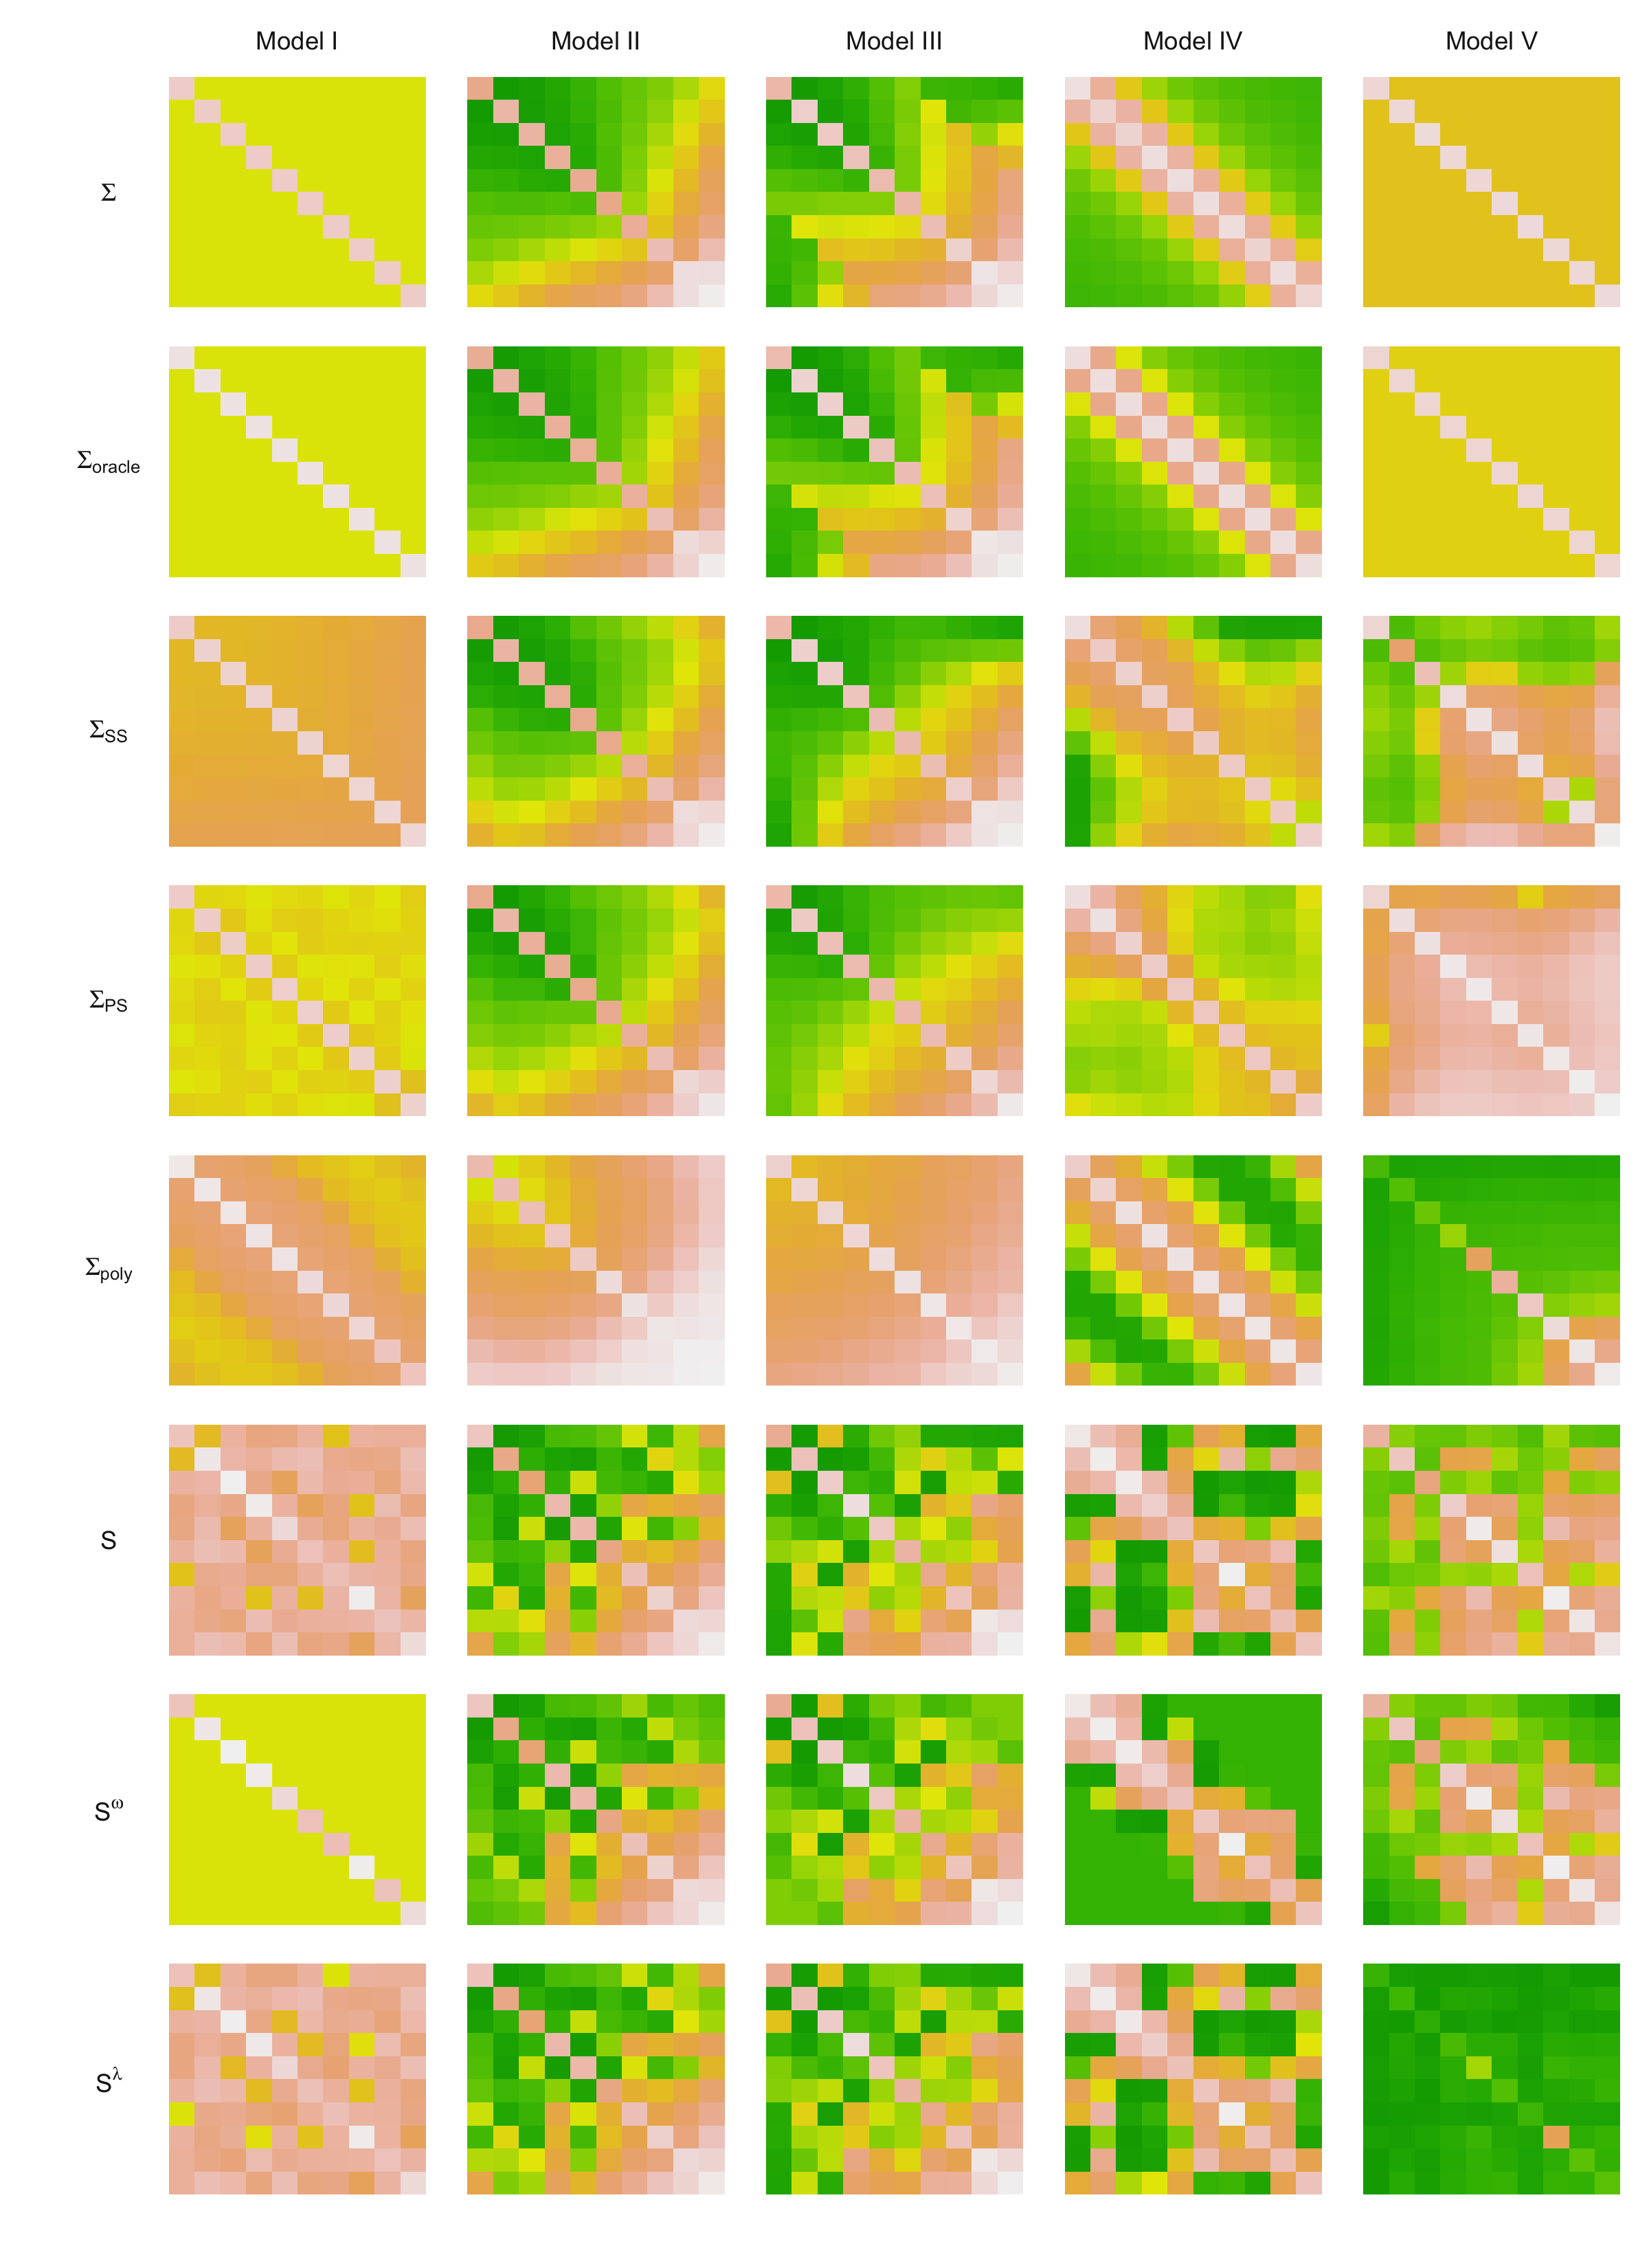
\includegraphics[width = 1\textwidth]{../img/chapter-4/cov-estimate-lattice}\label{fig:cov-estimate-lattice}
\end{figure}

\begin{figure}[H] 
\centering
\caption{The true lower triangle of Cholesky factor $T$ corresponding to Model~\ref{item:cov-type-1} - Model~\ref{item:cov-type-5} and estimates of the same surface for estimators based on the modified Cholesky decomposition. The true covariance structure is displayed across the top row.}
  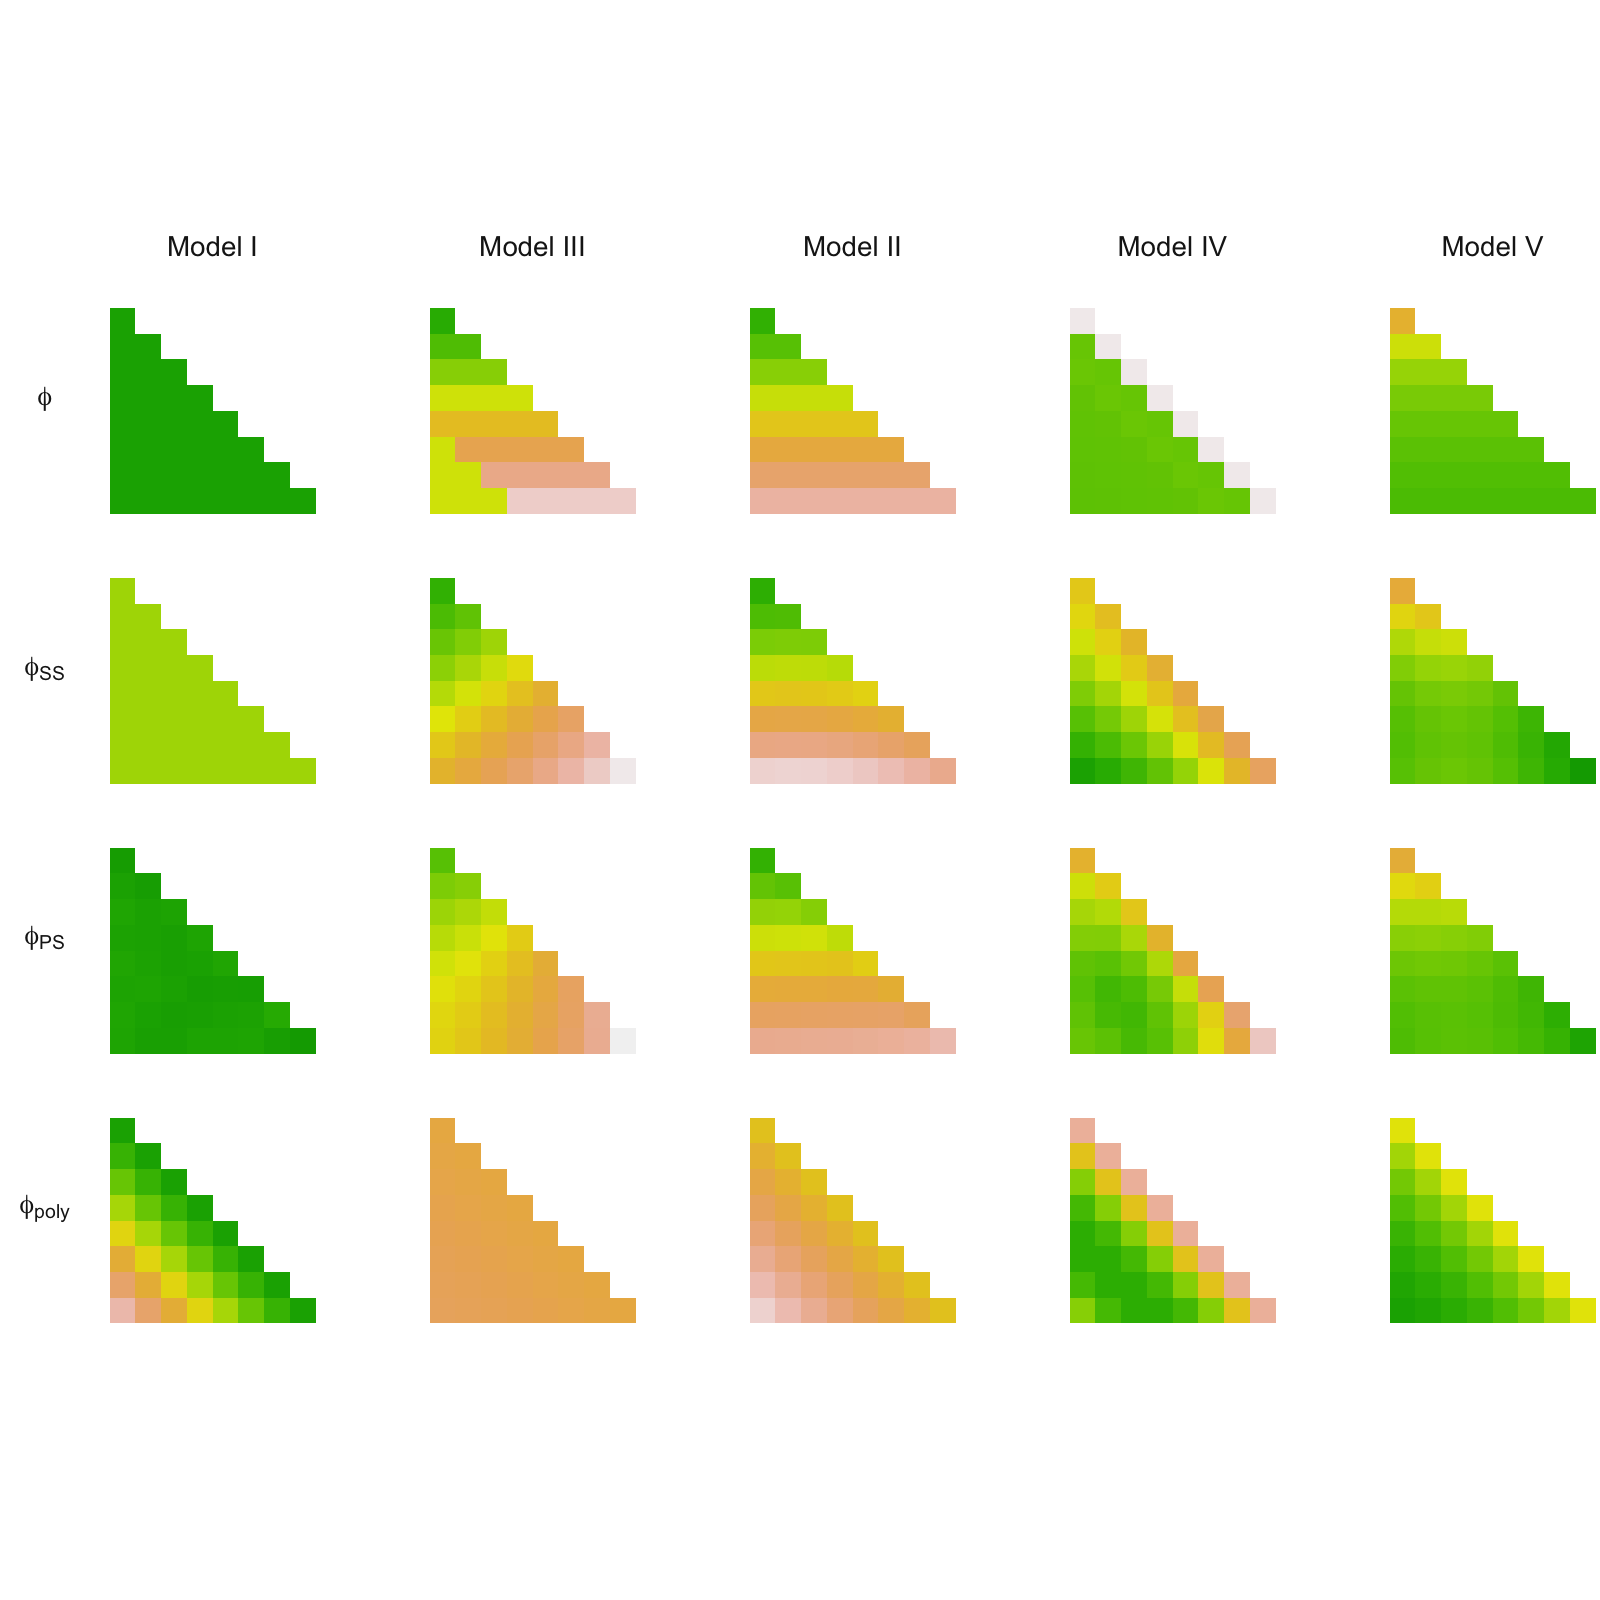
\includegraphics[width = 1\textwidth]{../img/chapter-4/cholesky-estimate-lattice}
  \label{fig:chol-estimate-lattice}
\end{figure}

%\subfile{chapter-4-subfiles/chapter-4-ssanova-lattice-ggplot}

\begin{figure}[H] 
\caption{Estimated functional components of the smoothing spline ANOVA decomposition $\phi = \phi_1 + \phi_2 + \phi_{12}$ for $\hat{\Sigma}_{SS}$ under each simulation model I - V.}
  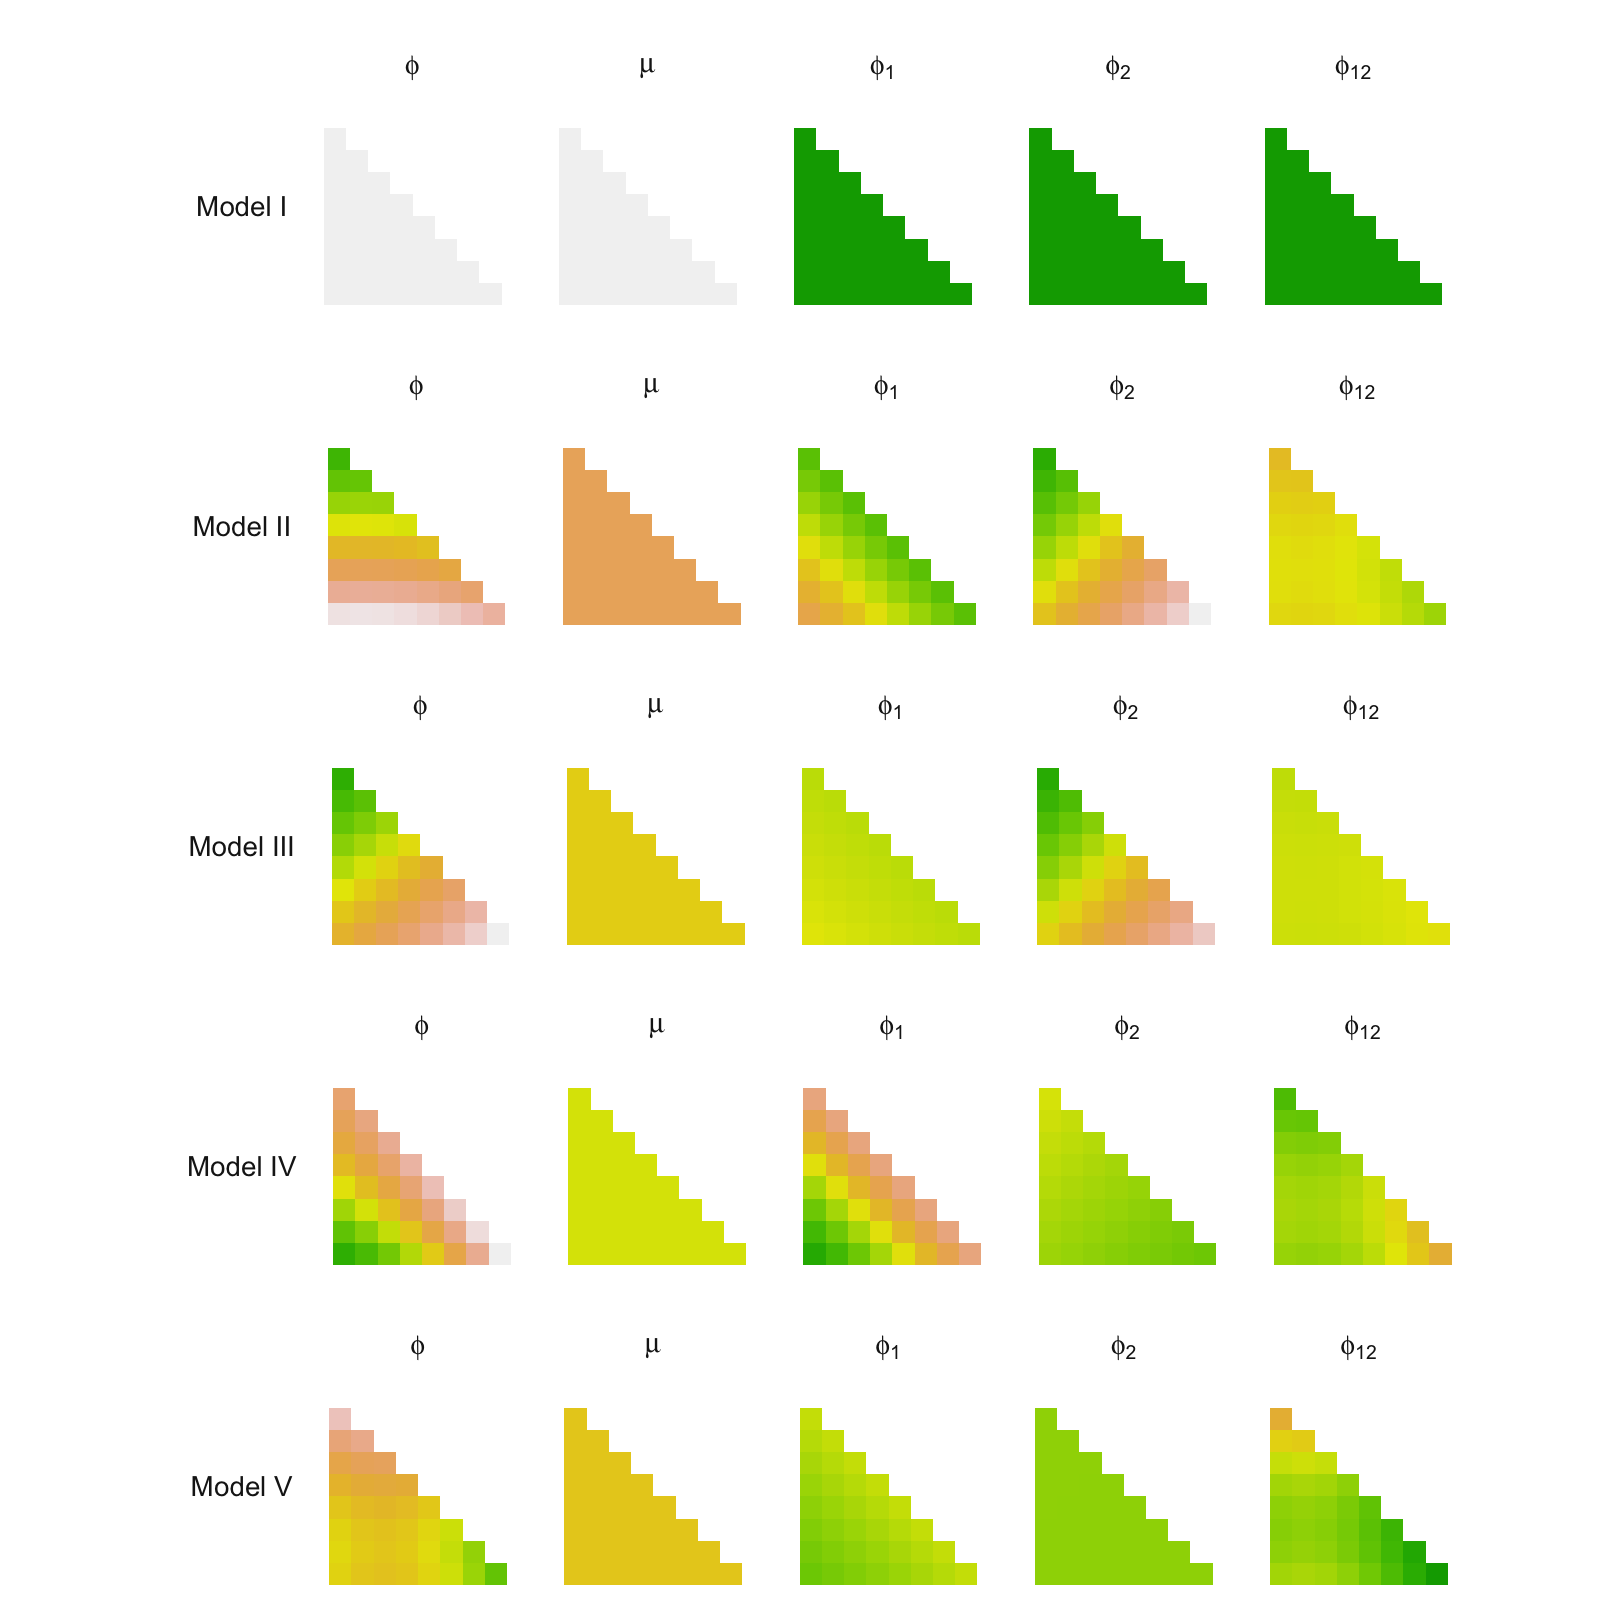
\includegraphics[width = \textwidth]{../img/chapter-4/ssanova-estimate-lattice} \label{fig:ssanova-component-lattice}
\end{figure}

\bigskip
Given covariance matrix $\Sigma$, risk estimates are obtained from$N_{sim} = 100$ samples from an $M$-dimensional multivariate Normal distribution with mean zero and the same covariance.  The results of the simulations for complete data under entropy loss are presented in Tables~\ref{table:simulation-1-entropy-loss-sigma-1} - \ref{table:simulation-1-entropy-loss-sigma-5}. Risk estimates under quadratic loss, while there is not agreement between results every time, qualitatively, they are similar in nature to those with entropy loss. These are left to the Appendix, Tables~\ref{table:simulation-1-quad-loss-sigma-1}-\ref{table:simulation-1-quad-loss-sigma-5}. Since both loss functions are not standardized, they cannot be compared across dimensions $M$.

\bigskip

%Our estimator is stable across all of the underlying covariance  structures for the differing number of sampled trajectories $N = 50, 100$, while the performance of the alternative estimators markedly improves when the subject sample size is doubled for each of the generating structures, particularly for the case of $M = 30$. Irrespective of tuning parameter selection method, our estimator is preferable to all three of the alternative estimators, except under Model IV when $N$ is large and within-subject sampling rates are moderate. Under this model, both the inverse covariance as well as the covariance matrix itself are sparse. Specifically, the inverse is banded so that $\sigma^{ij} = 0$ for $\vert i - j \vert > 1$, but the non-zero elements are quite large. Inversion results in a covariance matrix which decays quickly as distance from the main diagonal increases, which is in concordance with the assumed structure of the soft thresholding estimator. 

\bigskip

In general, our estimators outperform the alternative estimators across the five covariance structures. This is not surprising; the soft thresholding estimator assumes no ordering of the variables of the random vector, which all but one of the generating structures exhibit. The tapering estimator assumes that the absolute value of the covariance decays as $l$ increases; only model IV satisfies this. The parametric estimator based on the modified Cholesky decomposition assumes that $\phi$ can be modeled as a univariate function of $l$, which does not hold for any of the models, save model IV.

\bigskip

The smoothing spline estimator outperforms the P-spline estimator in cases where the underlying covariance structure cannot be modeled as a multiplicative function of $l$ and $m$ - namely, model II. The P-spline estimator outperforms the smoothing spline estimator under model IV, likely due to the advantage of trivially change the order of the difference penalty. When the difference order is specified so that the generating model belongs to the null space $\hilbert_0$, the search for the optimal set of smoothing parameters is a much easier task.   
 
\bigskip


%Review of generalized thresholding estimators, including the soft thresholding estimator is presented in in \ref{subsubsection:chapter-1-sss-1-3-4}. Recall that  $S^\lambda$ can be written as the solution to the optimization problem
%
%\begin{equation} \label{eq:soft-thresholding-objective-function}
%\mathpzc{s}_\lambda\left( z \right)  = \argmin{\sigma} \left[ \frac{1}{2} \left(\sigma - z\right)^2 + J_\lambda\left(\sigma \right)\right],
%\end{equation}
%\noindent
%so that estimation of the covariance matrix can be accomplished by solving multiple univariate Lasso-penalized least squares problems. 
%
\bigskip

\setlength{\dashlinedash}{0.5pt}
\setlength{\dashlinegap}{1pt}
\setlength{\arrayrulewidth}{0.2pt}
\subfile{chapter-4-subfiles/simulation-study-1-entropy-table-model-1}
\subfile{chapter-4-subfiles/simulation-study-1-entropy-table-model-2}
\subfile{chapter-4-subfiles/simulation-study-1-entropy-table-model-3}
\subfile{chapter-4-subfiles/simulation-study-1-entropy-table-model-4}
\subfile{chapter-4-subfiles/simulation-study-1-entropy-table-model-5}

%\subfile{chapter-4-subfiles/simulation-study-1-entropy-single-table}

Tuning parameter selection for the regularized versions of the sample covariance matrix was performed using cross validation. Under certain conditions pertaining to the ratio of sample sizes of the training and validation datasets, the $K$-fold cross validation criterion is a consistent estimator of the Frobenius norm risk. It is defined 

\begin{equation} \label{eq:K-fold-matrix--cv}
\mbox{CV}_F\left(\lambda \right) = \argmin{\lambda} K^{-1} \sum_{k = 1}^K  \vert \vert\hat{\Sigma}^{\left(-k\right)} - \tilde{\Sigma}^{\left(k\right)}  \vert \vert_F^2, 
\end{equation}
\noindent
%where $\tilde{\Sigma}^{\left(k\right)}$ is the unregularized estimator based on based on $\mathcal{D}_k$, and $\hat{\Sigma}^{\left(-k\right)}$ is the regularized estimator under consideration based on the data after holding $\mathcal{D}_k$ out.  Using this approach, the size of the training data set is approximately $\left(K - 1 \right)N/K$, and the size of the validation set is approximately $N/K$ (though these quantities are only relevant when subjects have equal numbers of observations). For linear models, it has been shown that cross validation is asymptotically consistent is the ratio of the validation data set size over the training set size goes to 1. See \citet{shao1993linear}. This result motivates the reverse cross validation criterion, which is defined as follows:
%
%\begin{equation} \label{eq:K-fold-matrix-reverse-cv}
%\mbox{rCV}_F\left(\lambda \right) = \argmin{\lambda} K^{-1} \sum_{k = 1}^K  \vert \vert\hat{\Sigma}^{\left(k\right)} - \tilde{\Sigma}^{\left(-k\right)}  \vert \vert_F^2, 
%\end{equation}
%\noindent
%where $\tilde{\Sigma}^{\left(-k\right)}$ is the unregularized estimator based on based on the data after holding out $\mathcal{D}_k$, and $\hat{\Sigma}^{\left(k\right)}$ is the regularized estimator under consideration based on $\mathcal{D}_k$. 
There is little established about the optimal method for tuning parameter selection in for the class of estimators based on element-wise shrinkage of the sample covariance matrix.  However, based on the results of an extensive simulation study presented in \citet{fang2016tuning}, we use $K = 10$-fold cross validation to select the tuning parameters for both the tapering estimator $S^\omega$ and the soft thresholding estimator $S^{\lambda}$. They authors implement cross validation for a number of element-wise shrinkage estimators for covariance matrices in the \citet{CVTuningCov} R package, which was used to calculate the risk estimates for $S^{\omega}$ and $S^{\lambda}$. 

\bigskip

As discussed in Chapter 1, in the limit, soft thresholding produces a positive definite estimator with probability tending to 1 (\citet{rothman2009generalized}), however element-wise shrinkage estimators of the covariance matrix, including the soft thresholding estimator, are not guaranteed to be positive definite. We observed simulations runs which yielded a soft thresholding estimator that was indeed not positive definite.  In this case, the estimate has at least one eigenvalue less than or equal to zero, and the evaluation of the entropy loss \ref{eq:entropy-loss} is undefined. To enable the evaluation of the entropy loss, we coerced these estimates to the ``nearest'' positive definite estimate via application of the technique presented in \citet{cheng1998modified}.  For a symmetric matrix $A$, which is not positive definite,  a modified Cholesky algorithm produces a symmetric perturbation matrix $E$ such that $A + E$ is positive definite.

\bigskip

\citet{pan2003modelling} present an iterative procedure for estimating coefficient vectors $\lambda$, $\gamma$ of the polynomial model \ref{eq:mcd-polynomial-model}. Their algorithm uses a quasi-Newton step for computing the MLE under the multivariate normal likelihood. Their work is  is implemented in the JMCM package for \textsf{R}, which we used to compute the polynomial MCD estimates.  For implementation details, see \citet{pan2017jmcm}. 	 



\bigskip